\documentclass[conference,compsoc]{IEEEtran}

\usepackage{graphicx}
\usepackage[utf8]{inputenc}
\usepackage[spanish, mexico]{babel}
\usepackage{csquotes}
\usepackage{enumitem}

% citations
\usepackage{biblatex}
\addbibresource{references.bib}

% graphics config
\graphicspath{{img/}}


% Information for title page
\title{Arquitectura Autónoma Descentralizada Orientada a Servicios para sistemas críticos}
\author{\IEEEauthorblockN{Bruno Campos Uribe}
\IEEEauthorblockA{0223329@up.edu.mx}}


\begin{document}

\maketitle

\begin{abstract}
    Un sistema distribuido es una colección elementos de computación autónomos que aparecen al usuario como un único sistema coherente. Esto se logra con la colaboración de estos elementos que se comunican entre ellos. Arquitectura Autónoma Descentralizada Orientada a Servicios es un mecanismo basado en comunicación asíncrona diseñado para cumplir las necesidades de un sistema distribuido de alto rendimiento. Un cliente del sistema se puede conectar a uno o varios servidores que actúan como intermediarios para el envío y recepción de mensajes a otros clientes del sistema. Se realizó una calculadora distribuida basada en esta arquitectura.
\end{abstract}

\section{Introducción}

La arquitectura de un procesador convencional puede considerarse ``internamente distribuido''. Distintos dispositivos separados dentro del procesador son responsables de ciertas tareas específicas (operaciones aritméticas, registros, almacenamiento). Estos dispositivos se interconectan por vías de comunicación que transportan información y mensajes. Estas vías están literalmente cableadas, y los ``protocolos'' que utilizan para transportar información son específicos y rígidamente definidos. Reorganizar el esquema de distribución implica cambiar la arquitectura física del dispositivo. Este nivel de inflexibilidad ofrece ventajas en términos de velocidad de procesamiento y latencia de transferencia de información.

El desarrollo de dispositivos periféricos, que se limitaban a realizar tareas específicas y se conectaban a dispositivos de computación central, creó la necesidad de desarrollar protocolos por los que varios dispositivos pudieran comunicarse. La popularización de la computadora personal sólo aumentó esta necesidad. El conjunto de protocolos estándar ha evolucionado hacia formar un sistema operativo de red mundial. Cada vez son más irrelevantes el tipo de hardware, sistema operativo y arquitectura de red que utilizan dispositivos específicos, lo que hace que las herramientas para procesar la información requieran cada vez más flexibilidad y disponibilidad.
\cite{farley_1998}

\subsection{Sistemas Distribuidos}

Hoy en día utilizamos redes de miles de estaciones de trabajo y computadoras personales para hacer nuestro trabajo, en lugar de enormes procesadores centrales.
Esto significa un cambio en el paradigma sobre el que diseñamos programas de computadora. Debemos ser capaces de aprovechar nuestras redes de computadoras más pequeñas para trabajar de forma conjunta en tareas de mayor complejidad computacional.\cite{farley_1998} Estas computadoras suelen estar dispersas geográficamente, por lo que se suele decir que forman un \emph{sistema distribuido}. \cite{steen_tanenbaum_2017}

Un sistema distribuido debe cumplir dos características. La primera es que un sistema distribuido es una colección de elementos de computación, cada uno de los cuales debe comportarse independiente de los demás. Un elemento puede ser un dispositivo de hardware o un proceso de software. La segunda característica es que para el usuario (ya sea una persona u otra aplicación), un sistema distribuido debe parecer como un único sistema coherente. En un sistema coherente el conjunto de elementos funciona igual, independiente de dónde, cuándo y cómo se produzca la interacción entre un usuario y el sistema. Esto implica que los elementos autónomos tienen que colaborar. Cómo establecer esta colaboración constituye la clave del desarrollo de los sistemas distribuidos.\cite{steen_tanenbaum_2017}

El diseño de un sistema distribuido debe complir cuatro objetivos principales: debe hacer que los recursos sean fácilmente accesibles; debe ocultar el hecho de que los recursos están distribuidos a través de una red; debe ser abierto; y debe ser escalable. \cite{steen_tanenbaum_2017}

\subsubsection{Facilitar el intercambio de recursos}

Un objetivo importante de un sistema distribuido es facilitar el acceso y el uso compartido de recursos remotos. Los recursos pueden ser periféricos, instalaciones de almacenamiento, datos, archivos, servicios y redes, entre otros.

La conexión de usuarios y recursos también facilita la colaboración y el intercambio de información.

\subsubsection{Transparencia de distribución}

Un sistema distribuido intenta que la distribución de procesos y recursos sea transparente, es decir, invisible, para los usuarios finales.

\begin{table}[!h]
    \caption{\\Diferentes formas de transparencia en un sistema distribuido. Un objeto puede ser un recurso o un proceso\cite[][Figura 1.2]{steen_tanenbaum_2017}.}
    \label{tab:transparencia}
    \begin{tabular}{|l|p{2.25in}|}
        \hline
        \textbf{Transparencia} & \textbf{Descripción} \\ \hline
        Acceso & Ocultar las diferencias en la representación de los datos y la forma de acceder a un objeto. \\ \hline
        Ubicación & Ocultar dónde se encuentra un objeto. \\ \hline
        Reubicación & Ocultar que un objeto puede ser movido a otra ubicación mientras está en uso. \\ \hline
        Migración & Ocultar que un objeto puede moverse a otra ubicación. \\ \hline
        Réplica & Ocultar que un objeto está replicado. \\ \hline
        Concurrencia & Ocultar que un objeto puede ser compartido por varios usuarios independientes. \\ \hline
        Fallo & Ocultar el fallo y la recuperación de un objeto. \\ \hline
        \end{tabular}
\end{table}

\subsubsection{Ser abierto}

Un sistema distribuido abierto es un sistema que ofrece componentes que pueden ser fácilmente utilizados o integrados en otros sistemas.

\subsubsection{Escalabilidad}

\begin{samepage}
La escalabilidad de un sistema puede medirse en al menos tres dimensiones diferentes\cite{neuman1994scale}:

\begin{description}
    \item[Tamaño:] Un sistema puede ser escalable con respecto a su tamaño, lo que significa que podemos añadir fácilmente más usuarios y recursos al sistema sin que haya una pérdida de rendimiento.
    \item[Geografía:] Un sistema escalable geográficamente es aquel en el que los usuarios y los recursos pueden estar muy alejados entre sí, sin que los retrasos en la comunicación afecten la funcionalidad del sistema.
    \item[Administrativa:] Un sistema escalable desde el punto de vista administrativo es aquel que puede seguir siendo fácilmente gestionado aunque abarque muchas organizaciones administrativas independientes.
\end{description}
\end{samepage}

\subsection{Arquitectura}

Para asegurar el correcto funcionamiento de un sistema distribuido, es crucial sus elementos estén debidamente organizados. La organización de los sistemas distribuidos se refiere sobre todo a los componentes de software que constituyen el sistema. Estas arquitecturas de software nos indican cómo deben organizarse los distintos componentes de software y cómo deben interactuar.\cite{steen_tanenbaum_2017}

\subsubsection{Cliente-servidor}

En el modelo más sencillo de cliente-servidor, los procesos de un sistema distribuido se dividen en dos grupos. Un \emph{servidor} es un proceso que implementa un servicio específico. Un \emph{cliente} es un proceso que solicita un servicio a un servidor enviando una petición y espera posteriormente la respuesta del servidor\cite{steen_tanenbaum_2017}.

En esta arquitectura, el servidor se encarga de todo, mientras que el cliente no es más que un terminal mudo. Este es el modelo más sencillo de una \emph{arquitectura por capas}. Un enfoque para organizar los clientes y los servidores consiste en distribuir más de dos capas capas en diferentes máquinas. Sin embargo, se sigue haciendo una distinción entre sólo dos tipos de máquinas: las máquinas cliente y las máquinas servidoras, lo que conduce a lo que también se denomina una arquitectura (físicamente) de dos niveles\cite{steen_tanenbaum_2017}.

\begin{figure}[htb]
    \centering
    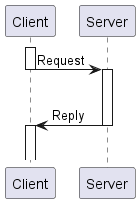
\includegraphics[width=0.35\columnwidth]{client-server.png}
    \caption{Interacción cliente-servidor.}
    \label{fig:client_server}
\end{figure}

\subsubsection{Arquitectura descentralizada}

Una distribución en capas es también conocida como una \emph{distribución vertical}. En contraste, en la \emph{distribución horizontal} un cliente o servidor se divide en partes lógicamente equivalentes, cada parte operando en su propia parte del conjunto de datos, equilibrando la carga de procesamiento\cite{steen_tanenbaum_2017}.

\subsection{Modelos de Interacción}

\subsubsection{Comunicación Síncrona}

Cuando se llama a un procedimiento en el modelo de síncrono, el código que llama debe bloquear y suspender el procesamiento hasta que el código llamado complete la ejecución y le devuelva el control; el código que llama puede ahora continuar el procesamiento. Cuando se utiliza el modelo de interacción síncrona los sistemas no tienen independencia de control de procesamiento; dependen de la respuesta de los sistemas llamados \cite{curry_2004}.

El modelo de comunicación síncrona también se ilustra en la Figura \ref{fig:client_server}.

\subsubsection{Comunicación Asíncrona}

El modelo de interacción asíncrona, ilustrado en la Figura \ref{fig:async}, permite a quien llama mantener el control del procesamiento. El programaque llama no necesita bloquearse y esperar a que el código llamado responda. Este modelo permite al elemento que llama continuar el procesamiento independientemente del estado de procesamiento del procedimiento llamado. Con la interacción asíncrona, el procedimiento llamado puede no ejecutarse inmediatamente. Este modelo de interacción requiere un intermediario para gestionar el intercambio de peticiones \cite{curry_2004}.

\begin{figure}[htb]
    \centering
    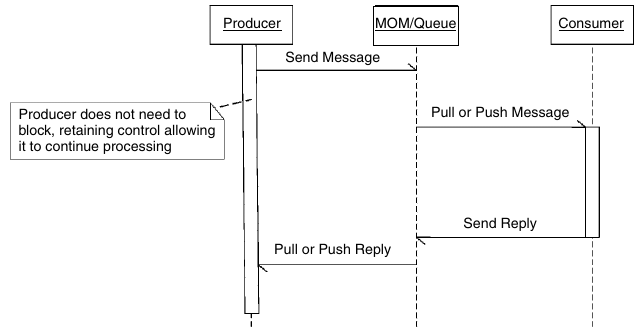
\includegraphics[width=\columnwidth]{async.png}
    \caption{Modelo de interacción asíncrono \cite[][Figura 1.2]{curry_2004}.}
    \label{fig:async}
\end{figure}

\subsection{Message-Oriented Middleware}

Los sistemas que operan entornos críticos con exigencias de disponibilidad 24/7, alto rendimiento, y alta integridad los sistemas tradicionales centralizados fracasan para cumplir estas necesidades.

Un mecanismo basado en comunicación asíncrona diseñado para cumplir con estas necesidades se conoce como \emph{Middleware Orientado a Mensajes} (MOM).\cite{curry_2004} Un cliente de un sistema MOM se conecta a uno o varios servidores que actúan como intermediarios para el envío y recepción de mensajes a y de otros clientes del sistema. Las plataformas basadas en MOM permiten crear sistemas flexibles y cohesivos.

Cuando se utiliza MOM, una aplicación emisora no tiene ninguna garantía de que su mensaje será leído por otra aplicación ni se le da una garantía sobre el tiempo que tardará el mensaje en ser entregado. Estos aspectos los determina principalmente la aplicación receptora\cite{curry_2004}.

\begin{figure}[t]
    \centering
    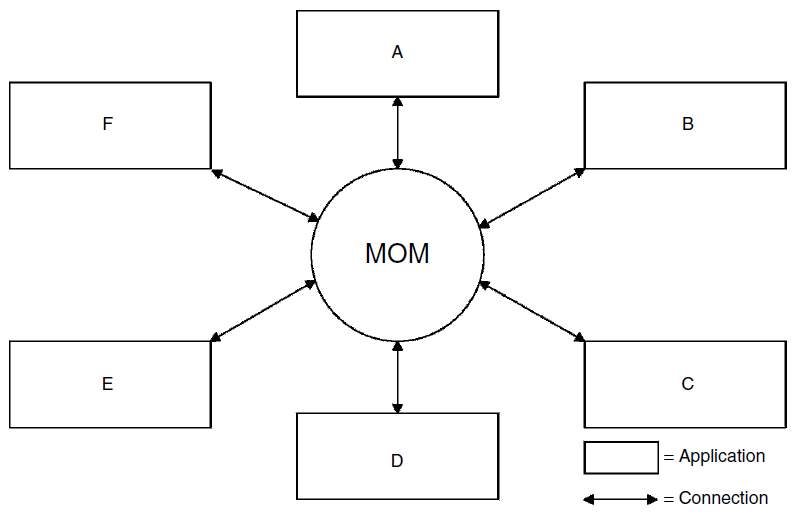
\includegraphics[width=\columnwidth]{mom.png}
    \caption{Diagrama de un sistema distribuido basado en MOM \cite[][Fig. 1.4]{curry_2004}.}
    \label{fig:mom}
\end{figure}

\subsubsection{Acoplamiento}

MOM inyecta una capa entre emisores y receptores. Esta capa independiente actúa como intermediaria para el intercambio de mensajes. El acoplamiento flexible entre los participantes de un sistema enlaza aplicaciones sin tener que adaptar los sistemas de origen y destino entre sí, lo que da lugar a un despliegue de sistemas altamente cohesivo y desacoplado\cite{curry_2004}.

\subsubsection{Confiabilidad}

Con MOM, la pérdida de mensajes por fallos de la red o del sistema se evita utilizando un mecanismo de almacenamiento y retransmisión para la persistencia de los mensajes. Esta capacidad de MOM introduce un alto nivel de confiabilidad en el mecanismo de distribución. El almacenamiento y retransmisión evita la pérdida de mensajes cuando partes del sistema no están disponibles o están ocupadas\cite{curry_2004}.

\subsubsection{Escalabilidad}

Además de desacoplar la interacción de los subsistemas, MOM también desvincula las características de rendimiento de los subsistemas entre sí. Los subsistemas pueden ampliarse de forma independiente, con poca o ninguna alteración de otros subsistemas. MOM también permite al sistema hacer frente a picos de actividad en un subsistema sin afectar a otras áreas del sistema. Los modelos MOM permiten balanceo de carga, al permitir que un subsistema elija aceptar un mensaje cuando esté preparado para hacerlo\cite{curry_2004}.

\subsection{Autonomous Descentralized Service Oriented Architecture}

La \emph{Arquitectura Autónoma Descentralizada Orientada a Servicios} (ADSOA) es una arquitectura que combina los conceptos de los \emph{Sistemas Autónomos Descentralizados}(ADS) y la \emph{Arquitectura Orientada a Servicios}(SOA). ADS fue propuesto para diseñar sistemas críticos de alta fiabilidad, expansibles y tolerante a fallos. Los sistemas en ADS están compuestos por subsistemas y entidades auto-administrados y auto-coordenados. Sin embargo, la implementación de un ADS suele requerir hardware y software especializado. Por lo tanto, ADSOA propone un modelo basado en ADS, utilizando conceptos de SOA para evitar el uso de hardware especializado.\cite{leguizamo_2017}

La arquitectura ADS está conformada por los siguientes componentes\cite{leguizamo_2017}:
\begin{description}
    \item[Entidad.] Un elemento que es una parte autónoma de la aplicación.
    \item[Canal de Datos.] Es el intermediario entre las entidades de la aplicación para el intercambio de mensajes.
    \item[Codigo de Contenido.] Es parte del protocolo de comunicación entre entidades. Cuando una entidad envía un mensaje, adjuntan un Código de Contenido. Las entidades conectadas aceptarán o descartarán el mensaje según los Códigos de Contenidos a los que estén registrados.
\end{description}

\section{Solución}

\begin{figure}[hbt]
    \centering
    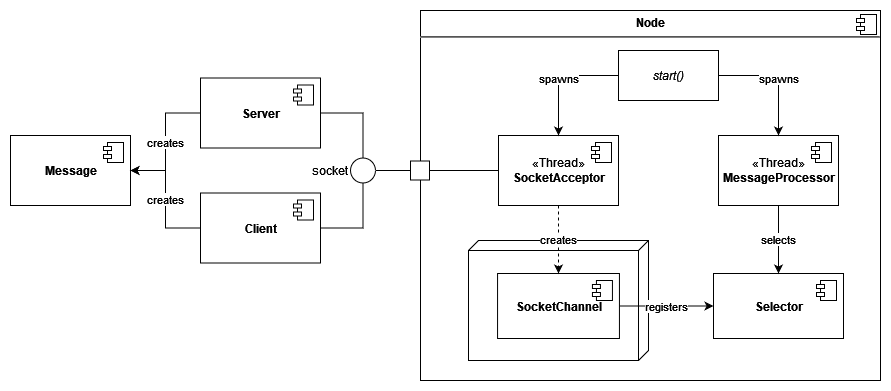
\includegraphics[width=\columnwidth]{node_components.png}
    \caption{Componentes del Nodo.}
    \label{fig:components}
\end{figure}

Se desarolló una calculadora utilizando una arquitectura ADSOA. Para implementar esta arquitectura se desarrollaron los siguientes compontentes, que se ilustran en la Figura \ref{fig:components}, que se describiran a detalle más adelante.

\begin{description}
    \item[Mensaje.] Encapsula el mensaje para enviar al Nodo. La estructura del mensaje incluye campos que lo identifican de manera única y permiten el filtrado por parte de las células. Los campos se detallan en la Sección \ref{sec:msg}
    \item[Nodo.] El Nodo es el elemento del canal datos que actúa como intermediario entre las células. Un Nodo mantiene una conexión a todos los demás nodos en la red, y se asegura de que un mensaje se propague a todas las Células.
    \item[Célula.] En el contexto de la arquitectura, una célula puede ser cualquier aplicación que se conectará al canal de datos para comunicarse con las otras células conectadas. Los distintos tipos de célula distinguen qué mensajes procesar o rechazar basado en su código de contenido.
    
    Para la calculadora se desarrollaron los siguientes tipos de célula:
    \begin{description}
        \item[Interfaz de Usuario.] Una interfaz gráfica que permite al usuario introducir operaciones y ver los resultados. También mantiene un registro de texto de todos los mensajes que salen y entran. La interfaz gráfica se muestra en la Figura \ref{fig:demo}.
        \item[Servidor.] El servidor es un manejador de servicios SOA. Recibe una operación de usuario, carga de manera dinámica la clase para evaluar la operación y envía el resultado.
    \end{description}
\end{description}

\subsection{Mensaje}\label{sec:msg}

El mensaje se encapsula en un registro inmutable con los siguientes campos, que también se muestran en la Figura \ref{fig:message}:
\begin{description}
    \item[contentCode] Código de Contenido. Los posibles códigos de contenido se describen en la Tabla \ref{tab:cc}.
    \item[requestUID] El identificador único de la célula que solicita la operación.
    \item[serviceUID] El identificador único de la célula que devuelve el resultado. Este campo sólo se usa cuando el código de contenido es \texttt{RES} o \texttt{ACK}, de lo contrario es nulo.
    \item[fingerprint] La clave única de evento. La clave se obtiene de los primeros 4 bits generados por un hash SHA-1 de la representación en bytes del código de contenido, el identificador del cliente, el contenido del mensaje y el índice de solicitud.
    \item[body] Un arreglo de bytes con el contenido del mensaje. Puede ser nulo.
\end{description}

El mensaje se serializa utilizando la interfaz \texttt{java.io.Serializable} para transmitirlo como un stream de bytes.

\begin{figure}[hbt]
    \centering
    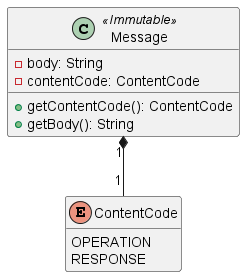
\includegraphics[width=0.9\columnwidth]{message.png}
    \caption{Diagrama de clase del Mensaje.}
    \label{fig:message}
\end{figure}

\begin{table}[hb]
    \centering
    \caption{Códigos de Contenido.}
    \label{tab:cc}
    \begin{tabular}{|l|l|l|}
    \hline
    \textbf{ContentCode} & \textbf{Descripción}              & \textbf{Receptor} \\ \hline
    \texttt{ADD}         & Operación de suma.                & Servidor          \\ \hline
    \texttt{SUB}         & Operación de resta.               & Servidor          \\ \hline
    \texttt{MUL}         & Operación de multiplicación.      & Servidor          \\ \hline
    \texttt{DIV}         & Operación de división.            & Servidor          \\ \hline
    \texttt{ACK\_ADD}    & Acuse de suma recibida.           & Interfaz          \\ \hline
    \texttt{ACK\_SUB}    & Acuse de resta recibida.          & Interfaz          \\ \hline
    \texttt{ACK\_MUL}    & Acuse de multiplicación recibida. & Interfaz          \\ \hline
    \texttt{ACK\_DIV}    & Acuse de división recibida.       & Interfaz          \\ \hline
    \texttt{RES}         & Resultado.                        & Interfaz          \\ \hline
    \end{tabular}
\end{table}

\subsection{Nodo}

Cuando se ejecuta el Nodo, escanea un rango de puertos proporcionados por el usuario (\texttt{50000-50100} por defecto) para iniciar un socket TCP de servidor. Después de vincular correctamente el puerto de servidor, vuelve a escanear el mismo rango de puertos para buscar otros Nodos existentes e intenta establecer una conexión para integrarse a la red interconectada del canal de datos.

El nodo inicia un hilo para procesar solicitudes de conexión. Cuando se registra una nueva conexión, espera que el remoto envíe un código de identificación para identificar la nueva conexión como una Célula u otro Nodo, y se registra en el Selector correspondiente para notificar un evento de escucha -- cuando hay un mensaje pendiente por recibir. Si el remoto envía un código de identificación no válido, o no envía el código de identificación en una ventana de 1 segundo, el Nodo termina la conexión.

Dos hilos concurrentes procesan los mensajes de los selectores. Si el Selector de Células recibe un mensaje, el mensaje se propaga a todas las conexiones, a excepción de la que recibió el mensaje; si el Selector de Nodos recibe un mensaje, el mensaje se propaga sólo a las Células conectadas directamente al Nodo, ya que se asume que otro Nodo está propagando el mensaje en el canal de datos.

El nodo se implementó con la librería de comunicación asíncrona de Java \texttt{java.nio} \cite{java17NIO}.

\begin{figure}[htb]
    \centering
    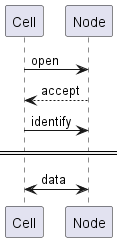
\includegraphics[width=0.3\columnwidth]{protocol.png}
    \caption{Protocolo de identificación.}
    \label{fig:protocol}
\end{figure}

\begin{table}[hb]
    \centering
    \caption{Códigos de Identificación.}
    \label{tab:handshake}
    \begin{tabular}{|c|l|}
    \hline
    \textbf{Código} & \textbf{Conexión} \\ \hline
    \texttt{'C'}    & Célula \\ \hline
    \texttt{'N'}    & Nodo \\ \hline
    \end{tabular}
\end{table}

\subsection{Células}

Cuando se executa una célula (Interfaz o Servidor), se intenta establecer una conexión TCP al primer Nodo disponible en un rango de puertos proporcionados por el usuario (\texttt{50000-50100} por defecto).

Cuando una célula recibe un mensaje del Nodo, puede decidir procesarlo o rechazarlo leyendo su código de contenido de acuerdo a la Tabla \ref{tab:cc}.

\begin{figure}[hbt]
    \centering
    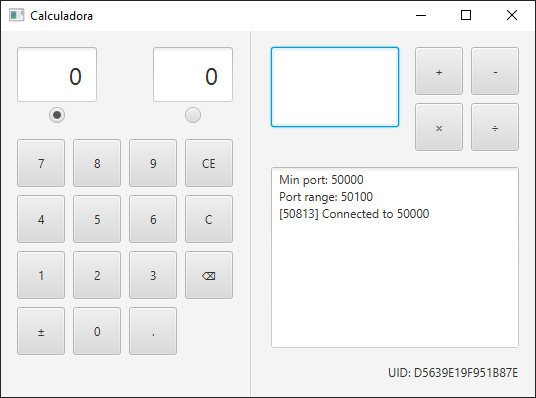
\includegraphics[width=0.9\columnwidth]{demo.png}
    \caption{Interfaz gráfica de la calculadora. Se puede observar en el registro el historial de comunicación con el Nodo al que está conectada.}
    \label{fig:demo}
\end{figure}

\subsubsection{Interfaz de Usuario}

Cuando el usuario inicia una operación, esta se enfila en una cola de procesamiento. Un hilo del programa monitorea el primer mensaje en fila y espera a recibir mensajes de acuse de un servidor. Para enviar la siguiente operación en cola, el programa debe recibir una cantidad determinada de acuses en un tiempo determinado (3 acuses en 1 segundo por defecto).

Cuando una interfaz recibe un mensaje de un nodo, primero verifica que la huella de solicitante coincida con su propia huella, de lo contrario descarta el mensaje.
Si el mensaje contiene un resultado, sólo lo mostrará al usuario si el mensaje con la misma clave ya tiene el número mínimo de acuses.

\section{Conclusiones}

La arquitectura ADSOA está diseñada para sistemas críticos donde el fallo de una entidad se considera una parte normal del sistema. ADSOA resuelve esto con un sistema redundante y auto-coordinado, que responda de manera dinámica al estado de todo el sistema.

%\newpage
\printbibliography

\end{document}
